\documentclass{article}
\usepackage{enumitem}


\usepackage{rotating}


\usepackage{listings}
\begin{document}

\begin{figure}[t]
\centering
	
\includegraphics[height=6.25cm,keepaspectratio]{Figures/logo}
\end{figure}

\title{TrackMe \\ Software Engineering 2 Project\\ \textit{ATD Document} }
\author{Stefano Martina, Alessandro Nichelini, Francesco Peressini
		\\ \\ A.Y. 2018/2019 \\ Version 1.1.0}
		
\maketitle
\newpage

\tableofcontents
\newpage

\section{Introduction}

\subsection{Purpose and Scope} 
The Acceptance Test Document has the purpose of evaluating the adherence of the implementation with respect to the  documents previously delivered.\newline
To do so, we have considered the three documents available in the provided repository.

\subsection{Reference} 
	As said above, we used the three documents, as referenced below:
	\begin{itemize}
		\item RASD Document : Requirements Analysis and Specification Document
		\begin{itemize}			\item v1.2 - 12/01/2019		\end{itemize}	
		\item DD Document : Design Document
		\begin{itemize}			\item v1.1 - 12/01/2019		\end{itemize}	
		\item ITD Document: Implementation and Testing Document
		\begin{itemize}			\item v1.0 - 13/01/2019		\end{itemize}	
	\end{itemize}
\subsection{Overview} 

\section{Project}
\subsection{Project info}


\newpage
\section{Installation Setup}
\subsection{Backend }
\subsubsection{Installation and launch}
	We have installed the backend as explained in the ITD Document, with the only exception of the particular system dependent command (we tested it on macOS).\newline
	We have installed the following module with \textit{"brew"} command:
	\begin{itemize}
		\item \textbf{PostgreSQL} an open source object-relational database system
		\begin{itemize}
			\item	installed with the command : \textit{brew install postgresql}
		\end{itemize}
		\item \textbf{NodeJS} an asynchronous event driven JavaScript runtime
		\begin{itemize}
			\item	installed with the command : \textit{brew install nodejs}
		\end{itemize}
	\end{itemize}
	After the launch of the postgres service with the command : \textit{brew services start postgresql}, we create a new database and a new role for the admin user. \newline
	Then, with the new role just created we import the dump of the database provided in the Implementation folder of the previously mentioned repository.
	As last step we have configured the \textit{"start.sh"} file with the following configuration and we launched it with the command \textit{"node app.js"}.
	\begin{figure}[h!]
		\centering
		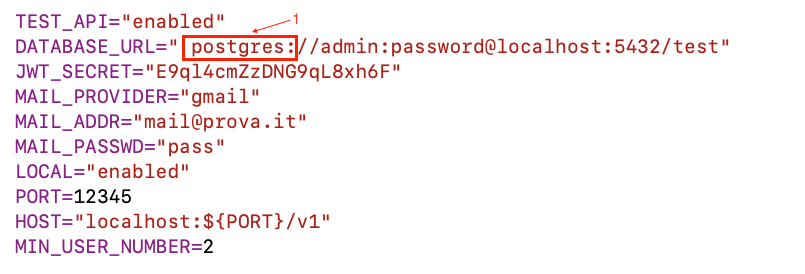
\includegraphics[height=4.25cm,keepaspectratio]{Figures/error1}
	\end{figure}
	
\subsubsection{Conslusion}
We didn't encounter particular issues, the guide lines are clear and enough explicative.\newline
The only thing which makes sense to be mentioned is one error encountered during the database connection. It always responds with "message: role //password// does not exists". This is due to a small error in the configuration file, probably due to the fact that is a machine dependant parameter (view image 1).

\newpage	
\subsection{Frontend - Installation and launch}
\subsubsection{Installation and launch}

\subsubsection{Conclusion}
	

\section{Acceptance Test}
\subsection{Issue}
\subsubsection{Issue1}
\subsubsection{Issue2}
\subsubsection{Issue3}


\subsection{Revision history}
\begin{itemize}
	\item 1.0.0 - Initial version (11/11/2018)

\end{itemize}
\subsection{Document Structure}

\newpage










\newpage
\section{Effort spent}

\begin{itemize}
	\item Stefano Martina: 35.00h
	\item Alessandro Nichelini: 37.00h
	\item Francesco Peressini: 37.00h
\end{itemize}

\end{document}